\chapter{Implementazione}\label{ch:implementazione}
\section{Scala 3}\label{sec:scala-3}
In questa sezione viene esaminato in che modo e dove sono stati utilizzati i nuovi costrutti di Scala 3 nel progetto.

\subsection{Impliciti}\label{subsec:impliciti}

\subsection{Macro}\label{subsec:macro}

\subsection{Context function}\label{subsec:context-function}

\subsection{Match types}\label{subsec:match-types}

\subsection{Type class}\label{subsec:type-class}

\subsection{Extension method}\label{subsec:extension-method}

\subsection{Problemi riscontrati}\label{subsec:problemi-riscontrati}
Nella libreria \texttt{scalatest} è stato riscontrato un bug nella sintassi \texttt{shouldNot typeCheck}.
Tramite questa espressione, dovrebbe essere possibile verificare che una porzione di codice, specificata come stringa,
non compili a causa di un errore nel processo di type checking.
Questo controllo risulta utile nel verificare la corretta destrutturazione delle~\texttt{CList} tramite pattern
matching.
In particolare si è verificato, tramite il codice riportato nel Listato~\ref{lst:lstinputlisting22}, che la
destrutturazione di una \texttt{CList} di dimensione diversa da quanto atteso porti ad un errore di compilazione.
a tal proposito si è definito il test indicato nel Listato~\ref{lst:lstinputlisting22}:
\lstinputlisting[label={lst:lstinputlisting22}, caption=Test per la verifica dell'unpacking delle CList.]
{./code/scalatest-bug.scala}
La prima asserzione verifica che la destrutturazione fallisca se si specificano meno elementi di quanti siano
effettivamente presenti nella lista;
nella seconda si testa lo scenario opposto, ovvero che la destrutturazione fallisca se la lista contiene meno elementi
di quanti ne sono stati specificati nel pattern matching.
Sebbene in entrambi i casi ci si aspetta che le espressioni non compilino a causa di errori nella fase di type checking,
questo non accade e le espressioni vengono erroneamente valutate come valide.
Il bug è stato segnalato agli sviluppatori della libreria mediante una issue~\cite{scalatest-bug}.

Sin dalle prime fasi di sviluppo si è abilitata la modalità di \textit{cross-building}~\cite{cross-building} affinché il
framework venisse compilato anche per Scala.js~\cite{scalajs}.
Questo ha generato una serie di falsi errori all'interno dell'IDE (IntelliJ);
infatti se si eseguivano i comandi di Sbt per la compilazione del progetto, quest'ultimo non sollevava alcun errore.
tanto è vero che se si eseguivano i comandi di Sbt per la compilazione del progetto, quest'ultimo non sollevava alcun
tipo di errore.
A tal proposito è stata aperta una issue~\cite{intellij-issue} sul bug tracker di Jetbrains.
Per una maggiore agilità nella scrittura del codice si è quindi scelto di rimuovere la \textit{cross-building} dal
progetto.

Si segnala che, essendo il rilascio di Scala 3 relativamente recente, non è stato possibile utilizzare
le seguenti librerie per problemi di compatibilità:
\begin{itemize}
    \item Scalafix
    \item Scoverage
    \item ScalaFXML
    \item ScalaMock
\end{itemize}

\section{Benchmarks}\label{sec:benchmarks}
Il requisito non funzionale~\ref{itm:nf1} richiede che il framework operi sotto certi requsiti di prestazioni;
per questo motivo è stato necessario quantificare oggettivamente quali fossero le effettive prestazioni raggiunte.
I benchmark sono uno strumento piuttosto efficace per valutare i tempi di esecuzione (e non solo), fornendo
una stima delle prestazioni in gioco.

Con il termine benchmark si intende un insieme di test specifici per misurare le prestazioni di un software o computer.
Al termine dell'esecuzione del benchmark si ottiene un indice indicativo delle prestazioni che il sistema in oggetto ha
raggiunto.
I benchmark possono essere raggruppati in due categorie:
\begin{itemize}
    \item Sintetici (o microbenckmark): vanno a misurare le prestazioni di alcune parti specifiche di un sistema
    \item Applicativi: misurano le prestazioni complessive di un sistema, ad esempio di un'applicazione
\end{itemize}

Dal momento che si vogliono valutare solo le prestazioni di una specifica parte del framework si è deciso di effettuare
dei microbenchmark.

Per implementare tali benchmark si è fatto uso del framework \texttt{Jmh}~\cite{jmh}, il quale consente di definire in
modo piuttosto semplice ma altamente configurabile i benchmark.

Scrivere benchmark che misurano correttamente le prestazioni di solo una piccola parte di software è difficile: ci sono
diverse ottimizzazioni che la JVM e l'hardware sottostante sono in grado di fare quando il benchmark esegue solo il
componente, ma tali ottimizzazioni non possono essere effettuate quando il componente è eseguito come parte dell'intera
applicazione, producendo dati falsati.
Implementazioni errate di benchmark possono far credere che le prestazioni dei componenti siano migliori di quanto non
lo siano in realtà.

Scrivere un benchmark corretto tipicamente evita che la JVM e l'hardware sottostante effettuino ottimizzazioni
durante l'esecuzione del benchmark, che invece potrebbero non essere effettuate a livello complessivo di
applicazione.
Grazie a Jmh tutte queste configurazioni sono fatte in automatico e gestite direttamente dal framework, consentendo di
concentrarsi solamente su cosa deve essere testato.

Mediante annotazioni su classi e metodi, è possibile configurare uno o più benchmark: nel
Listato~\ref{lst:lstinputlisting4} è possibile osservare un esempio di configurazione.

\lstinputlisting[label={lst:lstinputlisting4}, caption=Codice per eseguire il setup di un benchmark.]
{code/benchmark.scala}

Come è possibile osservare dal listato, Jmh fornisce molteplici configurazioni che possono essere apportate al
benchmark.
Di particolare rilevanza troviamo: \texttt{@Warmup} e \texttt{@Measurement}.

Con la prima si specifica quante iterazioni devono essere eseguite ``a vuoto'' prima d'iniziare con i test effettivi;
questa procedura risulta necessaria dal momento che quando si esegue per la prima volta un programma sulla JVM, la cache
risulta vuota e quindi il caricamento iniziale delle classi è più lento.
Eseguendo più volte la stessa porzione di codice si ``stabilizza'' la cache, quindi gli accessi successivi saranno più
veloci e uniformi.
Inoltre, nelle JVM HotSpot, l'interprete tiene traccia del numero di volte che un metodo viene eseguito: se tale
numero supera una certa soglia allora viene identificato come \texttt{hot method} (metodo che tipicamente ha dei
loop) e quindi \textit{JIT compiled}.
Chiamate successive all'ottimizzazione risulteranno quindi più veloci ed efficienti.
In questo modo si garantisce che le misurazioni successive alla fase di warm up abbiano valori simili senza essere
influenzate da condizioni esterne.

Con la seconda si specifica quante volte il benchmark debba essere ripetuto.
Per ogni esecuzione viene annotato il tempo impiegato e al termine dell'esecuzione viene riportato il tempo medio che
impiega il test.

\subsection{Risultati}\label{subsec:risultati}
Di seguito sono analizzati i risultati ottenuti dai benchmark delle \View e dei \System.
In Figura~\ref{fig:system} viene mostrato il grafico riguardante i \System in cui si può osservare che con $10000$
entità un sistema impiega mediamente cinque millisecondi ad aggiornare le entità, quindi il requisito~\ref{itm:nf1} è
ampiamente rispettato.

\begin{figure}[H]
    \centering
    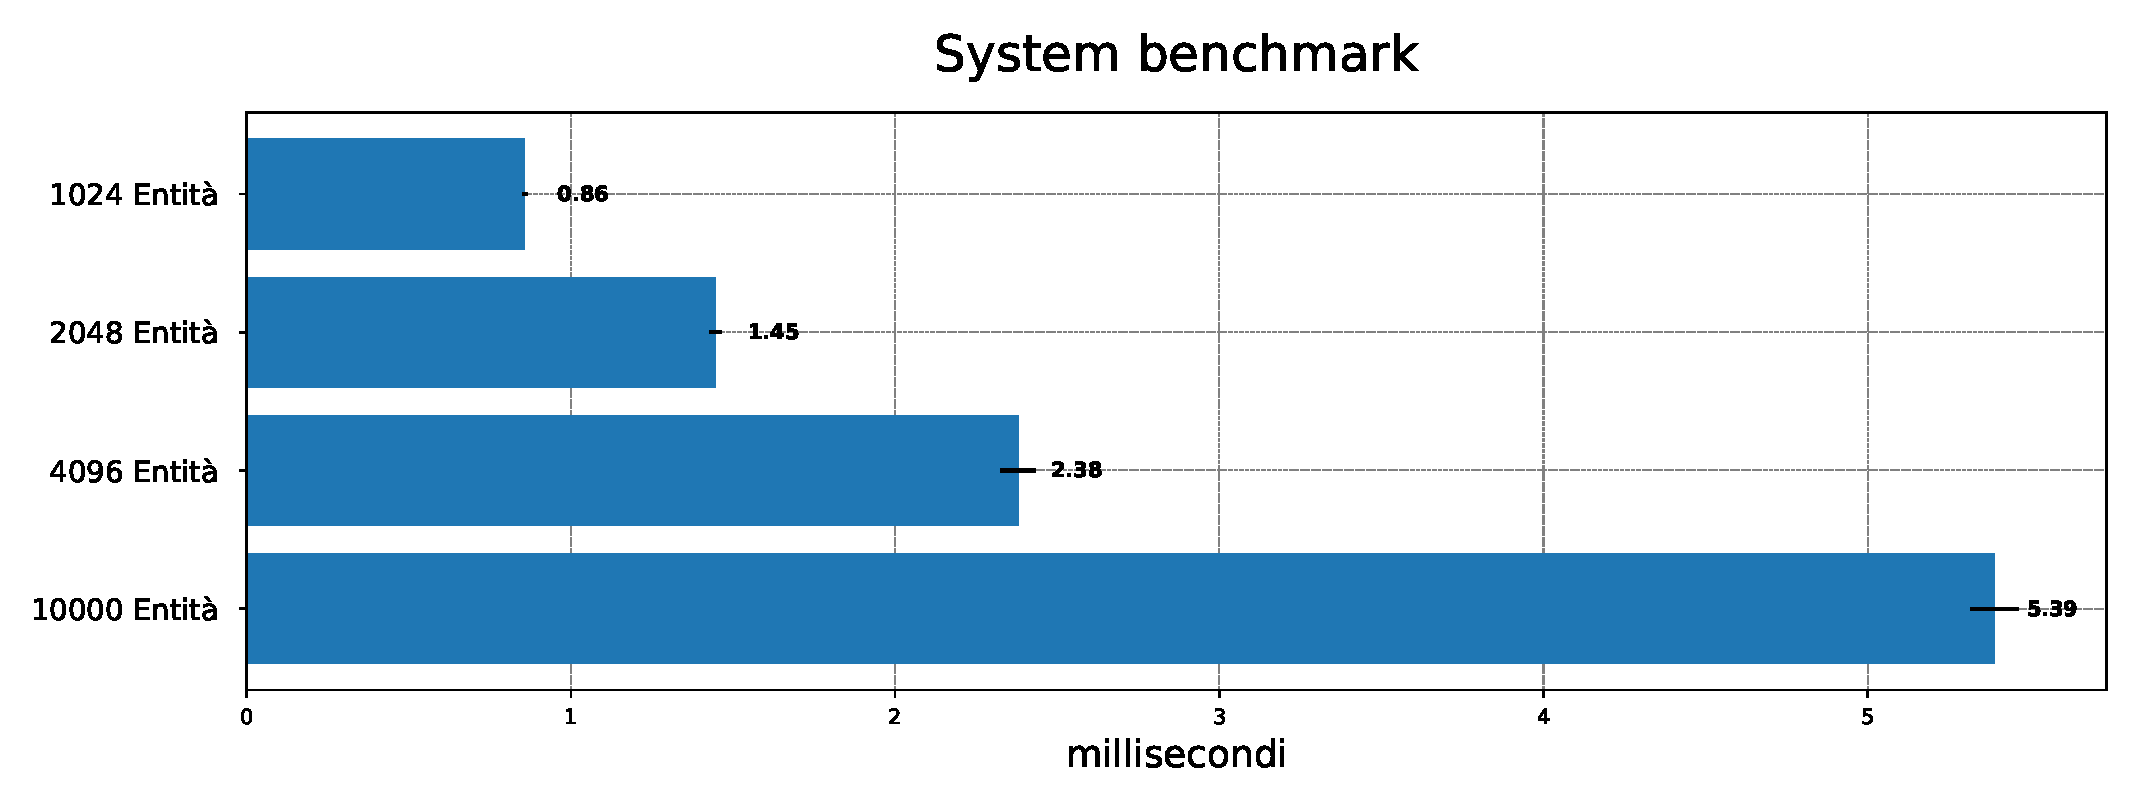
\includegraphics[width=\textwidth]{./img/system-benchmark}
    \caption{Tempi di esecuzione di un \System}\label{fig:system}
\end{figure}

A fronte dei risultati ottenuti dai benchmark si può affermare che il framework fornisce buone prestazioni con un numero
piuttosto elevato di entità.

\section{Suddivisione del lavoro}\label{sec:suddivisione-del-lavoro}
In questa sezione viene illustrata la suddivisione del lavoro e le parti di progetto realizzate da ciascun membro del
gruppo.

\subsection{Farabegoli}\label{subsec:farabegoli}
Il contributo apportato al progetto ha toccato buona parte del core del framework e della demo.
Mi sono infine occupato della gestione del repository, della \textit{Continuous Integration}, dei rilasci del framework
e della qualità del codice.

\subsubsection{Sviluppo collaborativo}
Spesso mi sono trovato a lavorare assieme ad altri membri del gruppo per risolvere problematiche o fornire spunti per
un migliore sviluppo del codice.
A tal proposito sono state frequenti le sessioni di lavoro in \textit{pair programming} che ci hanno consentito di
superare velocemente difficoltà nell'implementazione del codice, oltre a intercettare fin da subito potenziali bug.

\subsubsection{Component list}
Una caratteristica importante della libreria è quello di permettere di specificare nel tipo di un sistema (o una view)
su quali componenti questi operano, così che le stesse firme dei metodi possano guidare il programmatore indicando i
tipi dei componenti trattati.
Così facendo si elimina la necessità di specificare a tempo di esecuzione il tipo di componenti richiesto (come per
esempio è necessario fare nella libreria Ashely~\cite{ashley} che ricorre al passaggio di oggetti Class<?>)
permettendo di intercettare diversi errori a tempo di compilazione.
Realizzare tale funzionalità a livello di compilazione si è rivelato essere una sfida che ha richiesto l’implementazione
delle CList, nonché l’utilizzo di macro per modificare il comportamento del compilatore introducendo controlli
personalizzati (descritti in~\ref{subsec:macro}).
Una CList (abbreviazione di Components List) è essenzialmente una lista di elementi eterogenei che preserva informazioni
sul tipo di ciascun elemento in maniera simile ad una tuple.
Per esempio si osservi il Listato~\ref{lst:lstinputlisting2}: la lista che contiene
i componenti Position e Velocity avrà come tipo~\texttt{Position~\&:~Velocity~\&:~CNil}, permettendo di conoscere il
tipo e la posizione dei suoi elementi.

In Figura~\ref{lst:lstinputlisting2} viene mostrato un esempio di utilizzo delle \texttt{CList} nelle~\texttt{View}.
\lstinputlisting[label={lst:lstinputlisting2}, caption=Esempio di utilizzo delle CList.]{code/clist-usage.scala}

L’idea alla base di questa soluzione è ispirata dalle Heterogeneous List della libreria
Shapeless\cite{shapeless}; una differenza significativa sta nel fatto che la definizione di una CList impone un
limite ulteriore sul tipo dei suoi elementi: devono tutti essere sottotipi di Component, parte dell’implementazione è
riportata al listato~\ref{lst:lstinputlisting}.

\lstinputlisting[label={lst:lstinputlisting}, caption=Esempio di codice per implementare CList.]{code/clist.scala}

Nel contesto del framework si vuole aggiungere il vincolo tale per cui gli elementi presenti nelle \texttt{CList} siano
sottotipo di \Component.

Le \texttt{CList} rappresentano una parte fondamentale del framework realizzato, quindi è stato importante realizzare
diversi test (anche in collaborazione con i miei colleghi) per cercare d'individuare possibili errori.
Un esempio significato riguarda i test effettuati sulla corretta destrutturazione di una CList: in questo ambito si è
rilevato un bug nella suite scalatest;
per una trattazione dettagliata del problema si veda la Sezione~\ref{subsec:problemi-riscontrati}.

L'ordine dei tipi che definiscono una \texttt{CList} è fondamentale ai fini della computazione dei \System poiché se non
venisse rispettato si avrebbero inconsistenze di tipi che porterebbero a una condizione di errore che si vuole evitare.
Ciò consente nelle implementazioni dei \System o delle \View d'identificare a tempo di compilazione se la
\texttt{CList} che viene ritornata ha lo stesso tipo di quella dichiarata nel sistema;
se ciò non accadesse, il compilatore segnala un errore d'inconsistenza di tipi.
In questo modo garantiamo che un errato utilizzo delle \texttt{CList} venga intercettato a compile time, oltre a
preservare la semantica di utilizzo.

\subsubsection{World ed Entity}
Una delle parti che ho seguito nelle prime fasi di sviluppo è stata l'implementazione del \World e delle \Entity.
In particolare mi sono occupato di definire l'interfaccia di entrambe le classi e di fornire una prima implementazione
di base.
Ho quindi implementato il codice necessario affinché ogni \Entity avesse un identificativo univoco nel \World.
Infine, mi sono occupato dello sviluppo dei test per la verifica delle classi oggetto d'implementazione.

\subsubsection{View}
Ho definito e implementato parzialmente la classe~\View: in particolare, ne ho realizzato l'interfaccia e fornito una
prima implementazione.
Sempre seguendo un approccio TDD, ho realizzato anche i test necessari alla verifica del corretto funzionamento delle
classi sopra descritte.
Sempre nell'ambito dello sviluppo delle \View, Cavalieri e Di Domenico hanno sviluppato una macro per costruire la
\View in modo che operi sui componenti effettivi passati nel generico;
in questa fase ho contribuito fornendo consigli e suggerimenti per una migliore implementazione del codice.

\subsubsection{Benchmarks}
Come descritto nel requisito non funzionale~\ref{itm:nf1} indica una linea di base delle prestazioni che il framework
deve rispettare;
A tal proposito ho definito una serie di benchmark per misurare le prestazioni di \View, \System e dell'aggiornamento
del World.
Mediante questi benchmark è stato possibile validare il requisito non funzionale sulla base di dati oggettivi.
Per una descrizione più approfondita dei benchmark si faccia riferimento alla Sezione~\ref{sec:benchmarks}.
L'aspetto di type-safety che garantiscono le \texttt{CList} è dato dal fatto che tutti i suoi componenti siano sotto tipo
di~\Component, quindi se viene costruita una~\texttt{CList} che comprenda un tipo che non è sotto tipo di~\Component,
allora l'errore viene intercettato a compile-time.

\subsection{Di Domenico}\label{subsec:nicolò-di-domenico}

Il mio ruolo nel progetto è stato principalmente quello d'implementare le \texttt{View} e i \texttt{System}, nonché
applicare ove necessario eventuali ottimizzazioni per rispettare il requisito non funzionale \ref{itm:nf1}.

\subsubsection{View}

Essendo le \texttt{View} ed \texttt{ExcludingView} progettate come indicato in Figura~TODO, si è rivelato utile costruire un
iteratore astratto che permettesse di fattorizzare tutto il codice comune.
In particolare si noti come la \texttt{ExcludingView} itera su un sottoinsieme delle entità ritornare dalla stessa
\texttt{View}, che invece non esprime vincoli di esclusione di componenti.
Per questo motivo è stato creato il \texttt{BaseViewIterator}, che si occupa di recuperare dal
\texttt{ComponentsContainer} tutte le mappe che associano ciascuna entità all'istanza (se presente) del componente di
ciascun tipo.
Infine, partendo da tali mappe, si occupa di testare l'appartenenza alla view di ciascuna entità e, in caso affermativo,
estrarne tutti i componenti richiesti.

Una semplice ottimizzazione utilizzata per rendere più veloce l'iterazione di una \texttt{View} consiste nell'individuare
la mappa di componenti con meno elementi;
una volta trovata, si iterano tutte le entità contenute al suo interno e per ognuna si controlla che sia presente in tutte
le altre mappe.
In caso affermativo, si procede all'estrazione di tutti i suoi componenti richiesti.

\subsubsection{System}

Un \texttt{System} è un blocco di codice che può essere aggiunto al \texttt{World} e viene chiamato a ogni aggiornamento
di stato della simulazione.
Ogni \texttt{System} ha due metodi:
\begin{itemize}
    \item \texttt{shouldRun}: metodo booleano che indica se il \texttt{System} dev'essere eseguito
    \item \texttt{update}: metodo che contiene il codice arbitrario da eseguire
\end{itemize}

Su di esso sono stati costruiti \texttt{IteratingSystem} ed \texttt{ExcludingSystem}, due wrapper type-safe
rispettivamente per \texttt{View} ed \texttt{ExcludingView}.
Questi due sistemi definiscono i seguenti metodi:
\begin{itemize}
    \item \texttt{shouldRun}: metodo booleano che indica se l'\texttt{IteratingSystem} dev'essere eseguito
    \item \texttt{before}: metodo eseguito prima di iterare su tutte le entità con i componenti richiesti
    \item \texttt{update}: metodo eseguito per ciascuna entità contenente le operazioni da effettuare sui suoi
    componenti richiesti
    \item \texttt{after}: metodo eseguito dopo aver iterato su tutte le entità con i componenti richiesti
\end{itemize}

Il metodo \texttt{update} deve ritornare una \texttt{CList} dei nuovi componenti;
grazie all'utilizzo delle \texttt{CList} (descritte in dettaglio in TODO) verrà verificato a tempo di compilazione che i
nuovi componenti abbiano lo stesso tipo di quelli su cui opera il sistema.
Per permettere la cancellazione di alcuni dei componenti, è stato implementato un \textit{match type} chiamato
\texttt{Deletable[L~<:~CList]}, come mostrato nel Listato~\ref{lst:deletable};
il suo scopo è quello di permettere l'inserimento in ogni posizione della \texttt{CList} un componente speciale chiamato
\texttt{Deleted}: in tal caso il componente in quella posizione sarà cancellato.

\lstinputlisting[label={lst:deletable}, caption=Implementazione del tipo \texttt{Deletable[L~<:~CList]}]{./code/deletable.scala}

L'\texttt{ExcludingSystem} è completamente analogo all'\texttt{IteratingSystem}, in quanto cambia solo la \texttt{View}
usata per ottenere le entità sulle quali iterare.
Per una maggiore più approfondita sui benchmark si faccia riferimento alla Sezione~\ref{sec:benchmarks}.